
\documentclass{article}
\usepackage{amsmath} 
\usepackage{blindtext}
\usepackage[a4paper, total={6in,6in}]{geometry}
\usepackage{graphicx}
\begin{document}
\section{Introduction}
% \includegraphics[scale=0.2]{../gsplines.svg}
$f(\phi(u,v))=g(u,v)$

\begin{equation}
\label{eqn:G1}\phi(x,0)=(x,0)
\end{equation}

$\phi=(\phi_1,\phi_2)$

implies the folowing:

$y \,  divides \,\phi_2(x,y)$

ie

$\phi_2(x,y)=y.k(x,y)$

and:

$\phi_1(x,y)=x +y.q(x,y)$

for some polynomials $q,k$.

\section{Gk conditions}
the Gk are all the partial derivative of order less than k of $f(phi) $ and $g$ are equale.


\section{G1 Equation}

Because of the \ref{eqn:G1} the jacobian of $\phi$ is of the forme:

$$D\phi=
\begin{pmatrix}
1&a(u,v)\\
0 &b(u,v)
\end{pmatrix}
$$
a and b are functions of u,v.

and the G1 condition: $\partial _v g=a(u,v)\, \partial _u f (\phi)+b(u,v)\, \partial _v f (\phi)$  with $v=0$.
can also be written:
$$\partial _v g=(\partial _u f (\phi),\partial _v f (\phi)) \begin{pmatrix} a\\b\end{pmatrix}$$

\section{G2 condition}
when $ v=0$:
$$\partial ^2_vg=(a,b)(DDf)(\phi)\begin{pmatrix} a\\b\end{pmatrix}+Df(\phi) \partial_v\begin{pmatrix} a\\b\end{pmatrix}$$
$DDf $ is the hessian of $f$.

\section{Deduce gluing data from a surface}

\subsection{Gluing condition}
We use the following $G^1$ conditions:
can also be written:
$$c(\partial _v g)=(\partial _u f (\phi),\partial _v f (\phi)) \begin{pmatrix} a\\b\end{pmatrix}$$
\subsection{existantce of a solution}
After homogenisation, the polynomial solution exists according to hilbert theorem on syzygies.

\subsection{Practical case: $R^2$ domain}

In case of an $R^2$ domain.
 we multiply the G1 equation above by $\partial _uf$ we get
$$c(\partial_uf\times\partial _vg)=(\partial _uf\times\partial _vf )b$$

 we multiplyu the G1 equation above by $\partial _vf$ we get
$$c(\partial_vf\times\partial _vg)=(\partial _vf\times\partial _uf) a$$

Remark: in the RHS of the two equations $(\partial _vf\times\partial _uf)=-(\partial _uf\times\partial _vf )$.

RMK: one solution will be to take $c=(\partial _uf\times\partial _vf )$ and a,b will follow.
\subsection{Practical case: $R^3$ domain}
In case of an $R^3$ domain, we take $c=LCM(\partial _uf\times\partial _vf )$, and the reste will follow.

The other value of $c$ that can be tested $c=Prod(\partial _uf\times\partial _vf )$ product of all components of the vector.
\section{Computing the basis over a corresponding topology}

The G1 condition is a polynomial of variable u of degree $k=3* deg_uf$ at most.

by evaluating this polynomial at $k$ values, we get the system determining the $G1$ relations.

So we are looking for functions $F=\sum_{i,j} f_{i,j}B^{i,j}$ $G=\sum_{i,j} g_{i,j}B^{i,j}$, such that:

$$c(\partial _v g)=(\partial _u f (\phi),\partial _v f (\phi)) \begin{pmatrix} a\\b\end{pmatrix}$$

by suing this notation for the CP:
$$\begin{matrix}
g_{01}&g_{11}&g_{21}&g_{31}&g_{41}\\
f_{00}&f_{10}&f_{20}&f_{30}&f_{40}\\
f_{01}&f_{11}&f_{21}&f_{31}&f_{41}\\
\end{matrix}
$$
we get the folowing equation:
$$c\sum B^i_n(g_{i,1}-f_{i0})=a\sum B^{i-1}_{n-1}(f_{i0}-f_{i-1,0})+b\sum B^i_n(f_{i,1}-f_{i0})$$

 We can organize a system in the folowing way:

$M
\begin{pmatrix}
g_{01}\\g_{11}\\g_{21}\\g_{31}\\g_{41}\\
f_{00}\\f_{10}\\f_{20}\\f_{30}\\f_{40}\\
f_{01}\\f_{11}\\f_{21}\\f_{31}\\f_{41}\\
\end{pmatrix}
$

with $M$ contain $k$ lines (the number of sample points given above), each one given by:
$M{i,*}=(G_1, F_0,F_1)$
and 

$$G_1=
\begin{pmatrix}
c(p_k)B^0_n(p_k)& ...& c(p_k)B^n_n(p_k)&\\
\end{pmatrix}$$

$$F_0=
\begin{pmatrix}
c(p_k)B^0_n(p_k)+a(p_k)B^{0}_{n-1}+b(p_k)B^0_n(p_k)\\
\bigoplus _{i=1..n-1}c(p_k)B^i_n(p_k)-a(p_k)B^{i-1}_{n-1}+a(p_k)B^{i}_{n-1}+b(p_k)B^i_n(p_k)\\
c(p_k)B^n_n(p_k)-a(p_k)B^{n-1}_{n-1}+b(p_k)B^n_n(p_k)\\
\end{pmatrix}
$$

$$G_1=
\begin{pmatrix}
-b(p_k)B^0_n(p_k)& ...& -b(p_k)B^n_n(p_k)&\\
\end{pmatrix}$$

\end{document}
